% ==================================================
% @brief    模型的建立与求解
% ==================================================


\mcmSection{模型的建立与求解}

\mcmSubsection{问题1:通过解三角行求出多波束探测的覆盖宽度}

在问题1中,$\alpha$是测垂面与海底坡面的交线与水平面的夹角,实际上正是测坡角。也就是说,在问题一中,存在等式:

\begin{equation}
    \gamma = \alpha
\end{equation}

\begin{figure}[h]
    \centering
    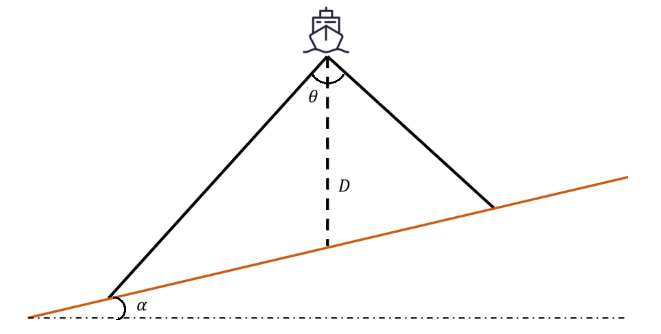
\includegraphics[scale=0.5]{res/img/探测船探测正视图.png}
    \caption{探测船探测正视图}
    \label{fig:探测船探测正视图}
\end{figure}

根据图\ref{fig:探测船探测正视图},为了求出覆盖宽度,可以抽象出如下的几何问题:

已知$\vartriangle PAB$是以$PA$、$PB$为腰的等腰三角形,其中,点$C$是$BP$上任意一点, PM是AB的垂线,且$\angle APB = \theta$, $\angle CAB = \gamma$, $PM = D$(如图\ref{fig:理想情况下的覆盖区域几何图}),求出$AC$在$AB$上的投影。

\begin{figure}[h]   
    \centering
    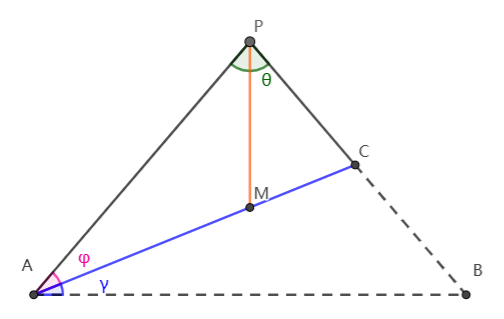
\includegraphics[scale=0.4]{res/img/理想情况下的覆盖区域几何图.png}
    \caption{\href{https://www.geogebra.org/m/xcvstdzg}{\textcolor{blue}{理想情况下的覆盖区域几何图}}}
    \label{fig:理想情况下的覆盖区域几何图}
\end{figure}

由题意可设$AM=x_1$,$MC=x_2$,$\angle PAM = \frac{\pi - \theta}{2} - \gamma = \varphi $.

对于$\vartriangle PAM$,根据正弦定理,存在方程:

\begin{equation*}
    \frac{\sin\angle APM}{AM} = \frac{\sin\angle PAM}{PM}
\end{equation*}

对于$\vartriangle PCM$,根据正弦定理,存在方程:

\begin{equation*}
    \frac{\sin\angle CPM}{CM} = \frac{\sin\angle PCM}{PM}
\end{equation*}

综上所述,将对应的值带入方程,可得下列方程组:

\begin{equation}
    \begin{cases}
        \varphi = \frac{\pi - \theta}{2} - \gamma \\
        \frac{\sin \frac{\theta}{2}}{x_1} = \frac{\sin\varphi}{D} \\
        \frac{\sin \frac{\theta}{2}}{x_2} = \frac{\sin(\pi-\theta-\varphi)}{D}
    \end{cases}
\end{equation}

解上述方程组以后,可得:

\begin{equation}
\begin{aligned}
    AC &= x_1 + x_2 \\
       &= \frac{\sin\frac{\theta}{2}}{\sin\varphi}D + \frac{\sin\frac{\theta}{2}}{\sin(\varphi + \theta)}D \\
       &= D\sin\frac{\theta}{2}\left(\frac{1}{\cos(\frac{\theta}{2}+\gamma)} + \frac{1}{\cos(\frac{\theta}{2}-\gamma)}\right)
\end{aligned}
\end{equation}

综上,可得如下结论:

\begin{mcmTheorem}{覆盖宽度公式}
    探测船的覆盖宽度$W$,与它的多波束换能器的开角$\theta$、测坡角$\gamma$、距离海底的深度$D$有关,满足如下等式:

    \begin{equation}
        W = 
        Proj AC = 
        D\sin\frac{\theta}{2}\left(\frac{1}{\cos(\frac{\theta}{2}+\gamma)} + \frac{1}{\cos(\frac{\theta}{2}-\gamma)}\right) \cdot \cos \gamma
        % \label{equ:覆盖宽度公式}
    \end{equation}
\end{mcmTheorem}

在问题一的情景中,当测量船与中心位置有一定偏移时,深度会发生改变,并且变化量$\Delta D$如图\ref{fig:深度变化}所示。



\begin{figure}[h]
    \centering
    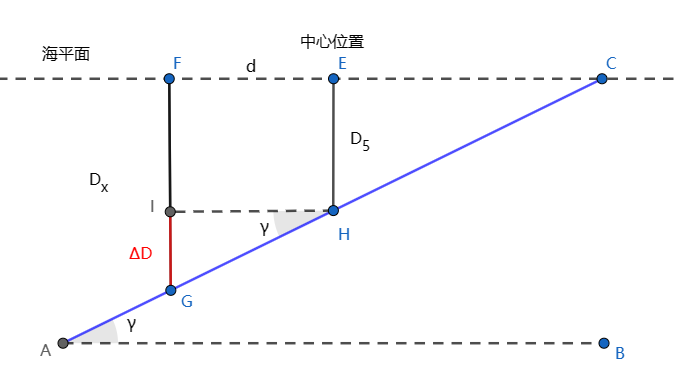
\includegraphics[scale=0.5]{res/img/深度变化.png}
    \caption{深度变化/TODO 添加超链接}
    \label{fig:深度变化}
\end{figure}

其中,线段$FC$是海平面,平行于线段$AB$,点$E$处是中心位置。为方便描述,设$\overrightarrow{FC}$、$\overrightarrow{EH}$分别为$x$轴、$y$轴正方向。

根据几何关系,易得:

\begin{equation}
    \Delta D = d\tan\alpha
\end{equation}

故中心距离\newline\newline\newline\newline

\begin{mcmTheorem}{海底深度函数}
    以海底深度由深到浅为正方向,确定某个中心位置$O$后,某个位置的深度$D(x)$与坡面坡度$\alpha$、中心位置的深度$D(0)$、与中心的距离$d$有关,满足如下公式:

    \begin{equation}
        D(d) = D(0) + d\tan\alpha
    \end{equation}
\end{mcmTheorem}

借原题中测线相互平行且海底地形平坦时的重叠率定义:

\begin{equation}
    \eta = 1 - \frac{d}{W}
\end{equation}

(其中$d$为相邻两条测线的间距,$W$为条带的覆盖宽度)

本文重新定义在均匀坡度下,当测线方向与海底坡面的法向在水平面上投影垂直时,重叠率为:

\begin{equation}
    \eta = 1-\frac{2d}{S_W}
\end{equation}

(其中$d$为相邻两条测线的间距,$S_W$为相邻两条条带的覆盖宽度之和)

当$\theta = 120^\circ$,$\gamma=\alpha=1.5^\circ$,海域中心点处的海水深度$D_5 = 70m$时,带入覆盖宽度公式和重叠率定义,得出下列结果:

% Please add the following required packages to your document preamble:
% \usepackage{booktabs}
\begin{table}[h]
    \centering
    \caption{\textbf{问题1的计算结果}}
    \begin{tabular}{@{}ccllllllll@{}}
    \toprule
    测线距中心点处的距离/$m$  & $-800$ & $-600$ & $-400$ & $-200$ & $0$ & $200$ & $400$ & $600$ & $800$ \\ \midrule
    海水深度/$m$        &      &      &      &      & 70  &     &     &     &     \\
    覆盖宽度/$m$        &      &      &      &      &   &     &     &     &     \\
    与前一条测线的重叠率/$\%$ &   -  &      &      &      &   &     &     &     &     \\ \bottomrule
    \end{tabular}
\end{table}


\mcmSubsection{问题二:一般情况下,覆盖率求解}

根据题意,可以抽象出如下的几何问题:

有两个直三棱柱如图\ref{fig:一般情况下的覆盖区域几何图}所示摆放,三棱柱$BEC-AFD$的侧边与三棱柱$DHC-FGE$的侧边相重合(这里用词是否准确?),其中,$AF$垂直于$FE$,$FG$垂直于$GE$,$\angle AFG=\beta$,$\angle CBE=\alpha$。设平面$ABCD$与平面$HCEG$的交线为$l_s$(图中未画出),求$l_s$与平面$ABEF$的夹角。

\begin{figure}[h]
    \centering
    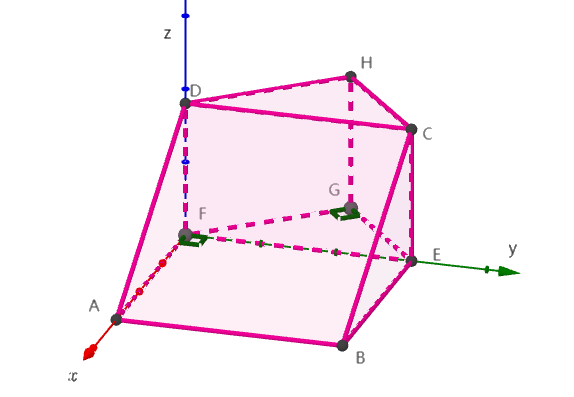
\includegraphics[scale=0.4]{res/img/一般情况下的覆盖区域几何图.png}
    \caption{\href{https://www.geogebra.org/m/absuxwpk}{\textcolor{blue}{一般情况下的覆盖区域几何图}}}
    \label{fig:一般情况下的覆盖区域几何图}
\end{figure}

分别设平面ABCD与平面HCEG的法向量为$\tau_\text{坡}$和$\tau_\text{测}$,$l_s$的方向向量为$v_s = (x_0, y_0, z_0)$.

根据平面法向量的性质,存在方程组:

\begin{equation}
    \begin{cases}
        \tau_\text{坡} \cdot v_s = 0 \\
        \tau_\text{测} \cdot v_s = 0
    \end{cases}
\end{equation}

又因为$\angle AFG=\beta$,$\angle CBE=\alpha$,可得:

\begin{equation}
    \begin{cases}
        \tau_\text{坡} = (\sin\alpha, 0, \cos\alpha) \\
        \tau_\text{测} = (\cos\beta, \sin\beta, 0)
    \end{cases}
\end{equation}

故有方程组:

\begin{equation}
    \begin{cases}
        x_0\sin\alpha + z_0\cos\alpha = 0 \\
        x_0\cos\beta + y_0 \sin\beta = 0
    \end{cases}
\end{equation}

即:

\begin{equation*}
    \begin{cases}
        y_0 = -x_0 \cot \beta \\
        z_0 = -x_0 \tan \alpha
    \end{cases}
\end{equation*}

不妨令$x_0 = -1$,则有:

\begin{equation}
    v_s 
    = (x_0, y_0, z_0)
    = \left( 
            -1,
            \cot \beta,
            \tan \alpha
      \right)
\end{equation}

因而:

\begin{equation*}
    \tan <l_s, ABEF> 
    = \frac {\tan \alpha} {\sqrt{(-1)^2 + \cot ^2 \beta}}
\end{equation*}

所以,$l_s$与平面$ABEF$的夹角为

\begin{equation}
    <l_s, ABEF> 
    = \arctan \left(|\sin \beta| \cdot  \tan \alpha\right)
    = \gamma
\end{equation}

\begin{mcmTheorem}{测坡角公式}
    \label{theorem:测坡角公式}
    对于一条测坡线$l_s$,$l_s$与水平面的夹角就是测坡角$\gamma$,$\gamma$与测线方向$\beta$、海底坡度$\alpha$有关,满足如下关系

    \begin{equation}
        \gamma = \arctan(|\sin\beta| \cdot \tan\alpha)
    \end{equation}
\end{mcmTheorem}

% Please add the following required packages to your document preamble:
% \usepackage{multirow}
\begin{table}[h]
    \centering
    \caption{问题2的计算结果}
    \begin{tabular}{cccccccccc}
    \hline
    \multicolumn{2}{c}{\multirow{2}{*}{覆盖宽度/m}} & \multicolumn{8}{c}{测量船距海域中心点处的距离/海里}        \\ \cline{3-10} 
    \multicolumn{2}{c}{}                        & 0 & 0.3 & 0.6 & 0.9 & 1.2 & 1.5 & 1.8 & 2.1 \\ \hline
    \multirow{8}{*}{测线方向夹角/°}       & 0         &   &     &     &     &     &     &     &     \\
                                    & 45        &   &     &     &     &     &     &     &     \\
                                    & 90        &   &     &     &     &     &     &     &     \\
                                    & 135       &   &     &     &     &     &     &     &     \\
                                    & 180       &   &     &     &     &     &     &     &     \\
                                    & 225       &   &     &     &     &     &     &     &     \\
                                    & 270       &   &     &     &     &     &     &     &     \\
                                    & 315       &   &     &     &     &     &     &     &     \\ \hline
    \end{tabular}
\end{table}

\mcmSubsection{问题三:为海域设计排线方案}

\mcmSubsubsection{方案设计与证明}

\textbf{确定测线的方向角$\beta$}

考虑一般情况,有以下简化模型:

假设有如下的直四棱柱$OBCD - O'B'C'D'$,其中$|OB| = l_{sea}$,$|OD| = w_{sea}$,$|OO'| = h$. 平面$BCEF$与平面$OBCD$之间的夹角为$\alpha$,$P$在交$O'B'$于点$A$,且$\angle B'AP = \beta$的射线上,且$|AP| = t$。需要求出代表船的点$P$在整个目标海域的条带总面积。计算过程如下:

\begin{figure}[h]
    \centering
    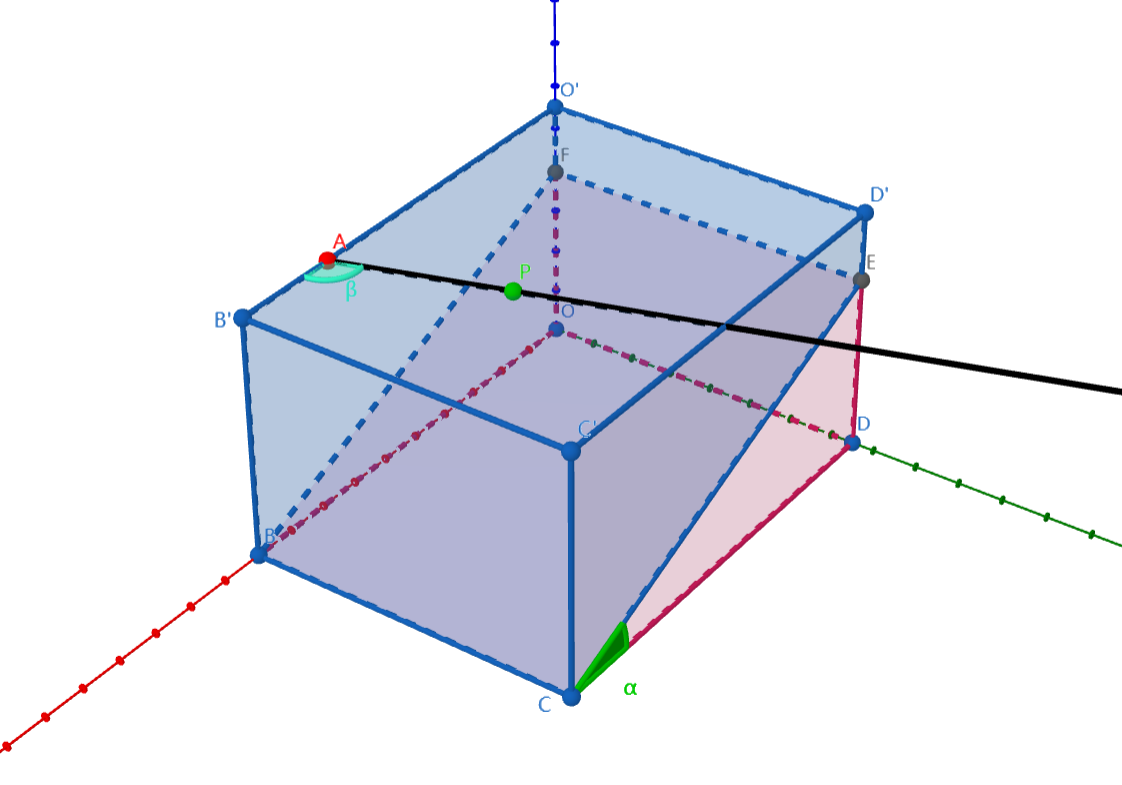
\includegraphics[scale=0.3]{res/img/一般情况下通式计算几何图.png}
    \caption{\href{https://www.geogebra.org/m/jzwhwcqr}{\textcolor{blue}{一般情况下通式计算几何图}}}
    \label{fig:一般情况下通式计算几何图}
\end{figure}

不难得出,坡面的解析式为:

\begin{equation}
    p: \ 
    (x - l_{sea})\tan \alpha + z = 0
\end{equation}

$A$点的坐标为:

\begin{equation}
    A = (l_{sea} - x, 0, h)
\end{equation}

由于单位向量$\tau_\text{测} = (\cos \beta, \sin \beta, 0)$,结合$|AP| = t$,可以得出$P$的坐标为:

\begin{equation}
    P = (l_{sea} - x + t\cos \beta, 
        t\sin \beta, 
        h)
\end{equation}

当前船(点$P$)的位置代入坡面解析式后,可以得出此时距离海水的深度的函数$D$的表达式为:

\begin{equation*}
    % D(\beta, x, t) = 
    % h - \left(l_{sea} - x\right)\tan \alpha
    D(\beta, t) = 
    h - \left(l_{sea} - x\right)\tan \alpha
\end{equation*}

即:

\begin{equation}
    % D(\beta, x, t) = 
    % h - \left(x - t\cos \beta \right)\tan \alpha
    D(\beta, t) = 
    h - \left(x - t\cos \beta \right)\tan \alpha
\end{equation}

由定理\ref{theorem:测坡角公式},根据船$P$当前的位置,可得测坡角函数$\gamma$的表达式为:

\begin{equation}
    \gamma(\beta) = 
    \arctan \left(|\sin \beta| \tan \alpha\right)
\end{equation}

由定理1,根据船$P$当前的位置,可得条带宽度函数$W$的表达式为:

\begin{equation}
    % w(\beta, x, t) = 
    % D(\beta, x, t)\cdot 
    % \left(
    %     \frac{1}{\cos (\frac{\theta}{2} + \gamma(\beta))} +
    %     \frac{1}{\cos (\frac{\theta}{2} - \gamma(\beta))}
    % \right)\cdot
    % \sin {\frac{\theta}{2}}\cdot \cos \gamma(\beta)
    W(\beta, t) = 
    D(\beta, t)\cdot 
    \left(
        \frac{1}{\cos (\frac{\theta}{2} + \gamma(\beta))} +
        \frac{1}{\cos (\frac{\theta}{2} - \gamma(\beta))}
    \right)\cdot
    \sin {\frac{\theta}{2}}\cdot \cos \gamma(\beta)
\end{equation}

此时,对自变量$t$定积分即可求得代表船的点$P$在整个目标海域的条带总面积,即总面积$S$的函数表达式为:

\begin{equation}
    % S(\beta, x) = 
    % \int _{0} ^{R(\beta, x)} {
    %     w(\beta, x, t)dt
    % }
    S(\beta) = 
    \int _{0} ^{R(\beta)} {
        W(\beta, t)dt
    }
\end{equation}

其中$R(\beta)$函数表示$t$的取值上限,且有:

\begin{equation}
    % R(\beta, x) = \min\left(
    %     \left|\frac{x - l_{sea}}{\cos \beta}\right|, 
    %     \left|\frac{w_{sea}}{\sin \beta}\right|
    % \right)
    R(\beta) = 
    \begin{cases}
        \min \left \{
                \frac{x}{\cos \beta}, 
                \frac{w_{sea}}{\sin \beta}
            \right \}
        & \beta \in \left(0, \frac{\pi}{2} \right)\\
        w_{sea} & \beta = \frac{\pi}{2}\\
        \min \left \{
                \frac{x - l_{sea}}{\cos \beta}, 
                \frac{w_{sea}}{\sin \beta}
            \right \}
        & \beta \in \left(\frac{\pi}{2}, \pi \right) 
    \end{cases}
\end{equation}

为了让这一测线测得的条带宽度尽可能大, 考虑令条带面积的导数为零,得到使其最大的$\hat \beta$。即求解$\hat \beta$使得:

\begin{equation}
    \frac{dS(\hat \beta)}{d\beta} = 0
\end{equation}

/TODO 猜测:

不难得出,当$\hat \beta = \frac{\pi}{2}$时,有条带面积最大值为:

\begin{equation}
    S(\hat \beta) = 
    w_{sea} \cdot (h - x\tan \alpha) \cdot \left[
        \frac{1}{\cos \left(
            \frac{\theta}{2} + \alpha
        \right)} + \frac{1}{\cos \left(
            \frac{\theta}{2} - \alpha
        \right)}
    \right]\cdot \sin \frac{\theta}{2} \cdot \cos \alpha
\end{equation}

因此,当测线的方向角$\beta = \frac{\pi}{2}$时相对优秀。

\textbf{确定相邻测线间距$d$}

要使测量长度最短,在确定测线方向角的情况下,利用贪心的思想,尽可能控制覆盖率$\eta = 10\%$。这样可以在单测线的测量长度不变的情况下,使测线条数减小,进而减小测量长度。

/TODO 这里是不是可以推导公式(第$i$条测线与第$i+1$条测线之间的距离$d_i$)?

\textbf{方案总结}

在测线的方向角固定为$\beta = \frac{\pi}{2}$时,动态调整相邻两条测线的间距$d$,以在保证整个海域均被覆盖的同时,控制重叠率为$\eta = 10\%$。

\mcmSubsubsection{计算流程}

\textbf{第一步: 求出第一条测线的最优方案}

若要使得整体测线方案最优,根据动态规划的最优子结构思想,需要先计算出第一条测线的最优情况,再根据第一条测线推导出其他测线方案,就可保证后续规划的每一条测线都为最优情况,最终做到整体测线方案为最优方案。

而第一条测线的最优情况,只能在边界条件下达成。分别有两种方案:

方案一 在东边界设立第一条测线.即按图4所示,AM在AB上的投影等于测线在以东向西为正方向时东西方向上的坐标。

方案二 在西边界设立第一条测线。即按图4所示,MC在AB上的投影等于测线在以西向东为正方向时东西方向上的坐标。

通过观察易知,第一条测线因无上一条测线,无需满足重叠率要求,故其覆盖宽度越大,整体探测效率越高。因此根据方案一确立第一条测线才为最优方案。

设第一条测线在以东向西为正方向时东西方向上的坐标为$x_1$(米),设海域中心在在以东向西为正方向时东西方向上的坐标为$W_c$(米),设海域中心点处的海水深度为$D_c$(米),则按图4模型可列方程:

\begin{equation}
    (W_c - x_1) \tan\alpha+D_c = \frac{x_1\sin \phi}{\sin \frac{\theta}{2} \cos \alpha} 
\end{equation}

从而解得$x_i$,进一步算得第一条测线的水深$D_1$(米)与覆盖宽度$CW_1$(米),其中$\gamma = \alpha$:

\begin{equation}
    D_1 =  (W_c - x_1) \tan{\alpha} + D_c
\end{equation}

\begin{equation}
    CW_1 = D_1\sin\frac{\theta}{2}\left(\frac{1}{\cos(\frac{\theta}{2}+\gamma)} + \frac{1}{\cos(\frac{\theta}{2}-\gamma)}\right) \cdot \cos \gamma
\end{equation}

\textbf{第二步: 进一步推导其他测线方案}

得到第一条测线的位置与覆盖宽度后,便可推出下一条测线的最优情况。

问题三要求所规划的整体测量长度最短,且相邻条带之间的重叠率满足 10\%~20\% 的要求。故意味着下一条最优测线与上一条最优测线的重叠率为10\%。设第$i$条测线在以东向西为正方向时东西方向上的坐标为$x_i$(米),水深为$D_i$(米),覆盖宽度为$CW_i$(米),故根据式(8)可列方程如下:

\begin{equation}
    1-\frac{2(x_i-x_{i-1})}{CW_{i-1}+CW_i} = 0.1
\end{equation}

\begin{equation}
    CW_i = D_i\sin\frac{\theta}{2}\left(\frac{1}{\cos(\frac{\theta}{2}+\gamma)} + \frac{1}{\cos(\frac{\theta}{2}-\gamma)}\right) \cdot \cos \gamma
\end{equation}

\begin{equation}
    D_i =  (W_c - x) \tan{\alpha} + D_c
\end{equation}

联立式(27)、式(28)、式(29),最终可解得$x_i$的值,即可确定下一条测线的最优方案。

循环执行第二步,并设立边界条件$ x <= 2W_c $,即可求出一组测量长度最短、可完全覆盖整个待测海域的测线。

\mcmSubsubsection{计算结果}



\mcmSubsection{问题四:在已有数据情况下的测线方案设计}

\begin{figure}[h]
    \centering
    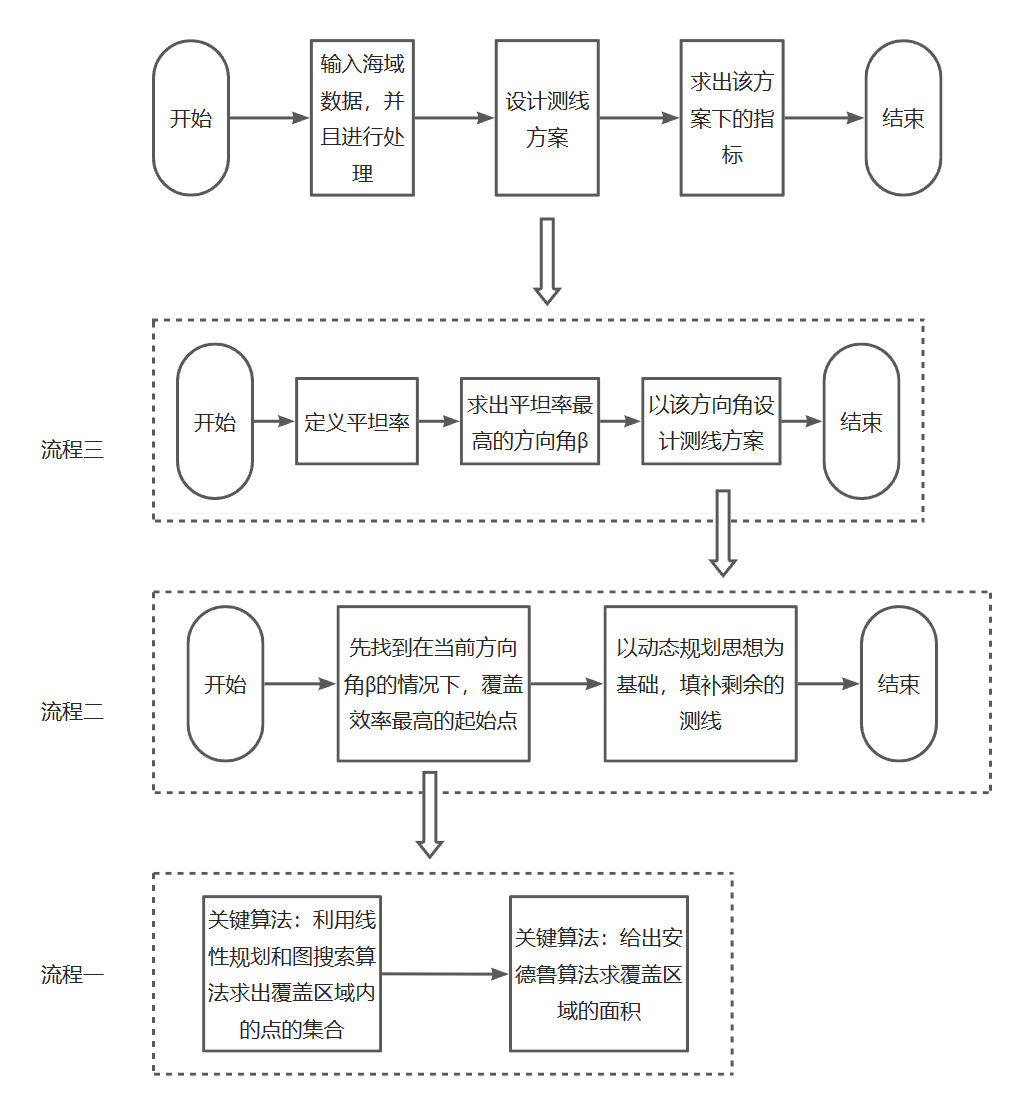
\includegraphics[scale=0.3]{res/img/第四问解答的算法流程图.png}
    \caption[short]{第四问解答的算法流程图}
\end{figure}

\mcmSubsubsection{第一步: 求出最优的测线方向角}

根据问题三的证明,为了尽可能保证每条测线的覆盖率最小,同时航行路程最短,应该尽可能让航行条带等宽。因此,在探测平坦的海底坡面时,只要尽力保证测线上每个点的深度不变即可。而为了为衡量这该不变程度,接下来定义海底坡面的平坦率$\varepsilon$。

首先定义某条测线的平坦率。在某条测线的海域下,从起点A到终点B之间的海底深度$D$的方差称为线段AB在该海域上的的平坦率。而对于问题四中给出的离散数据而言,应找到线段AB附近位置的海底深度数据,依次近似求出该线段的平坦率。定义该数据列表为$D_{i}$,平坦率$\varepsilon$满足:

\begin{equation}
    \varepsilon = \frac{1}{n} \sum^{n}_{i=1}(D_i - \overline{D} ) 
\end{equation}

其中,$\overline{D}$为深度的平均值。

而对于海底坡面的

接下来,枚举出全部方向上的平坦率,得到最优解

综上,得到一个测线方案

接下来,以(0,0)为初始位置,令$\beta = \frac{k}{72}\pi$,其中$k = 0, 1, \cdots, 36$,求出在该方向下的平坦率,如下表所示:



\mcmSubsubsection{第二步:求出最优测线方案}

在上述所有的方向中,平坦率最大值所对应的方向$\hat \beta$,认为是测线方向最合适的。随后,以该方向为基础,每间隔$d$增加一条测线,延伸到海域外围为止。随后,计算所有测线的平坦率。若有$n$条测线,对于第$i$条测线,其平坦率设为$\varepsilon_i$,并且所有测线平坦率对应的平均值,视为整个海域的平坦率,则有:

\begin{equation}
    \overline{\varepsilon} = \frac{1}{n} \sum^{n}_{i=1}\varepsilon_i 
\end{equation}

\mcmSubsubsection{第三步:求出最优测线方案下的各种指标}

首先,根据三维线性规划,求出某条测线能够覆盖的点的集合。

其次,将点集映射到水平平面后,根据安德鲁算法(凸包算法)求出该点集的轮廓,进而求出面积。同时与相邻测线的点集再取交集,以求出该交集的凸包的面积,为之后求覆盖率做准备。

最后,根据前面的计算过程,得出覆盖率。

% ==================================================
% @brief    模型的评价与改进
% ==================================================

\mcmSection{模型的评价与改进}